\documentclass{article}
\usepackage[a4paper]{geometry}
\usepackage{fancyhdr} 
\usepackage{tikz}
\usepackage{amsmath} 
\pagestyle{fancy}
\lhead{Winkel}
\rhead{Juli 2025}
\begin{document}
   
\newcommand{\norm}[1]{\big| {#1} \big|}  
\newcommand{\vect}[1]{\overrightarrow{#1}} 
  
\section{Winkel}
\subsection{Zwischen zwei Vektoren} 
\begin{minipage}[t]{\dimexpr\textwidth-3cm} 
Sind zwei Vektoren, $\vect{a}$ und $\vect{b}$, mit einem Winkel $\alpha$ gegeben, ist es offensichtlich, dass
\[
 \vect{a} = \begin{pmatrix} \norm{\vect{a}} \\ 0 \end{pmatrix}
 \quad \text{und} \quad 
 \vect{b} = \begin{pmatrix} \cos(\alpha) \norm{\vect{b}} \\ \sin(\alpha) \norm{\vect{b}} \end{pmatrix}
\]
Demnach folgt
\end{minipage} 
\hfill
\begin{minipage}[t]{3cm} 
 \centering 
 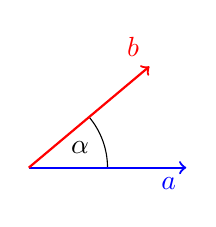
\begin{tikzpicture}[baseline=(current bounding box.north)]
  \coordinate (mid) at (0,0); 
  \path (mid) ++(2, 0) coordinate (enda);
  \path (mid) ++({2*sin(50)}, {2*cos(50)}) coordinate (endb);
 
  \draw (mid) ++(1, 0) arc[start angle=0, end angle=40, radius=1]; 
  \draw (mid) ++(0.65, 0.25) node {$\alpha$}; 
 
  \draw[->, thick,blue] (mid) -- (enda) node [below left] {$\vect{a}$};
  \draw[->, thick,red] (mid) -- (endb) node [above left] {$\vect{b}$};
 \end{tikzpicture} 
\end{minipage}
\begin{align*}
 \vect{a} \cdot \vect{b} &= \norm{\vect{a}} \cdot \cos(\alpha) \norm{\vect{b}} - \sin(\alpha) \norm{\vect{b}} \cdot 0 \\
 &= \norm{\vect{a}} \cdot \norm{\vect{b}} \cdot \cos(\alpha) \\
 \cos(\alpha) &= \frac{\vect{a} \cdot \vect{b}}{\norm{\vect{a}} \cdot  
\norm{\vect{b}}} \\
 \alpha &= \cos\left({\frac{\vect{a} \cdot \vect{b}}{\norm{\vect{a}} \cdot  \norm{\vect{b}}}}\right)
\end{align*}
Dies gilt, wie andersweitig ausführlicher Bewiesen werden kann, für alle zwei Vektoren.
 
\subsection{Zwischen zwei Geraden} 
\begin{minipage}[t]{4cm}
 \centering 
 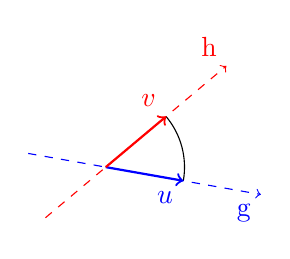
\begin{tikzpicture}[baseline=(current bounding box.north)]
  \coordinate (mid) at (0,0); 
  \path (mid) ++({-1*sin(100)}, {-1*cos(100)}) coordinate (startg);
  \path (mid) ++({2*sin(100)}, {2*cos(100)}) coordinate (endg);
  \path (mid) ++({-1*sin(50)}, {-1*cos(50)}) coordinate (starth);
  \path (mid) ++({2*sin(50)}, {2*cos(50)}) coordinate (endh);
  \path (mid) ++({1*sin(100)}, {1*cos(100)}) coordinate (endu);  
  \path (mid) ++({1*sin(50)}, {1*cos(50)}) coordinate (endv); 
 
  \draw (mid) ++(endu) arc[start angle=-10, end angle=40, radius=1];  
 
  \draw[->,blue,dashed] (startg) -- (endg) node [below left] {$\mathrm{g}$};
  \draw[->,red,dashed] (starth) -- (endh) node [above left] {$\mathrm{h}$};
  \draw[->,thick,blue] (mid) -- (endu) node [below left] {$\vect{u}$};
  \draw[->,thick,red] (mid) -- (endv) node [above left] {$\vect{v}$};
 \end{tikzpicture} 
\end{minipage} 
\hfill
\begin{minipage}[t]{\dimexpr\textwidth-4cm}
Werden beim Schnittpunkt von zwei Geraden jeweils ihre Richtungsvektoren eingezeichnet, wird offensichtlich, dass der Winkel zwischen den zwei Geraden auch der Winkel zwischen ihren beiden Richtungsvektoren ist. Haben die die beiden Geraden $\mathrm{g}$ und $\mathrm{h}$ die Richtungsvektoren $\vect{u}$ und $\vect{v}$, so ist der Winkel $\alpha$ 
\[
 \alpha = \cos\left({\frac{\vect{u} \cdot \vect{v}}{\norm{\vect{u}} \cdot  \norm{\vect{v}}}}\right)
\] 
\end{minipage}
  
\subsection{Zwischen Ebene und Gerade}   
\subsection{Zwischen zwei Ebenen} 
 
 
\end{document}
 
 
 
 
 
